\documentclass[cmpiitalkstyle, 25pt]{cmptalk}
\usepackage[utf8]{inputenc}

\hypersetup{pdfstartpage=1}%,pdfpagemode=FullScreen}%,pdfpagemode=None}
%\hypersetup{pdftitle=,pdfauthor=,pdfsubject=,pdfkeywords=}

\usepackage{bigfig,thumbpdf}
\usepackage[coloremph,display]{texpower}
%\usepackage[display]{texpower}
\usepackage{movie15}
%\usepackage{media9}

\newdimen\tmpd
\newbox\cmptalkverbbox

% notes customization (this one should be before begin document)
\cmptalkeverynotes={\usepackage{multicol}\usepackage{hyperref}\usepackage{movie15}}

\graphicspath{{../images/}}

%------------------------------------------------------------------- Title page
%-- specifications
\author{Pavel Trutman}
\affiliation{Centrum strojového vnímání}
\title{Generátor řešení minimálních problémů}
\acknowledgement{Vedoucí práce: Ing.\ Tomáš Pajdla, Ph.D.\\
Oponent: doc.\ Dr.\ Ing.\ Radim Šára}
\talklogo{
\includegraphics[width=4cm]{cmp}}

\begin{document}
\bigfigfalse
%\maketalktitlepage
\begin{talktitlepage}
  %\placeat{\Put(.5,.5){\thetalklogo}}
  \mbox{}\\
  {\Large\bfseries \thetitle }\\[\baselineskip]
  \theauthor \\[\baselineskip]
  %\begin{tabular}{rl}
  %  \textit{Vedoucí práce:}& \textit{Ing. Tomáš Pajdla, Ph.D.}\\
  %  \textit{Oponent:} & \textit{doc. Ing. Radim Šára, Dr. Tech.}
  %\end{tabular}
  \textit{Vedoucí práce: Ing.\ Tomáš Pajdla, Ph.D.}
  \vfill
  \thetalklogo\\[1cm]
  Centrum strojového vnímání\\
  Katedra kybernetiky\\
  Fakulta elektrotechnická\\
  České vysoké učení technické v Praze
  \vspace{2cm}
\end{talktitlepage}

% --------------------------------------------------------------------------- 
\begin{cmptalkslide}[Obsah]
  \begin{itemize}
    \item Motivace
    \item Automatický generátor
    \item Implementovaná vylepšení
    \end{itemize}
    \begin{narrow}[2]
    \begin{itemize}
      \item Víceeliminační postupy řešení
      \item Rozklad matic
      \item Algoritmus $F_4$
    \end{itemize}
    \end{narrow}
    \begin{itemize}
    %\item Benchmark Automatického generátoru
    \item Experimenty
  \end{itemize}
\end{cmptalkslide}

% --------------------------------------------------------------------------- 
\begin{cmptalkslide}[Motivace]
  \begin{itemize}
    \item Mnoho problémů v počítačovém vidění vede na řešení soustav polynomiálních rovnic
    \item Tyto soustavy je třeba řešit rychle $\rightarrow$ speciální postupy řešení
    \item Postupy řešení lze generovat automaticky $\rightarrow$ Automatický generátor \cite{AutoGen}
    \item Cílem je vylepšit Automatický generátor \cite{AutoGen}, aby generoval rychlejší a stabilnější postupy řešení
  \end{itemize}

  \placeat{
    \Put(0,0)[lb]{\footnotesize \cite{AutoGen} Z. Kukelova, M. Bujnak, T. Pajdla. Automatic generator of minimal problem solvers.}
  }

\end{cmptalkslide}

% --------------------------------------------------------------------------- 
\begin{cmptalkslide}[Automatický generátor]
  \begin{itemize}
    \item Z parametricky zadaných polynomiálních rovnic generuje postupy řešení, které umožňují tyto soustavy řešit pro konkrétní parametry
    \item Původní implementace \cite{AutoGen} generuje jednoeliminační postupy řešení
    %\item Systematicky generuje polynomy vyšších stupňů, dokuď nejsou vygenerovány všechny potřebné polynomy k extrakci řešení pomocí vlastních čísel a vektorů
    %\item Gauss-Jordanova eliminace
    %\item Sestavení multiplikativní matice
    %\item Extrakce řešení z vlastních vektorů multiplikativní matice
  \end{itemize}

  \placeat{
    \Put(.5,0.4){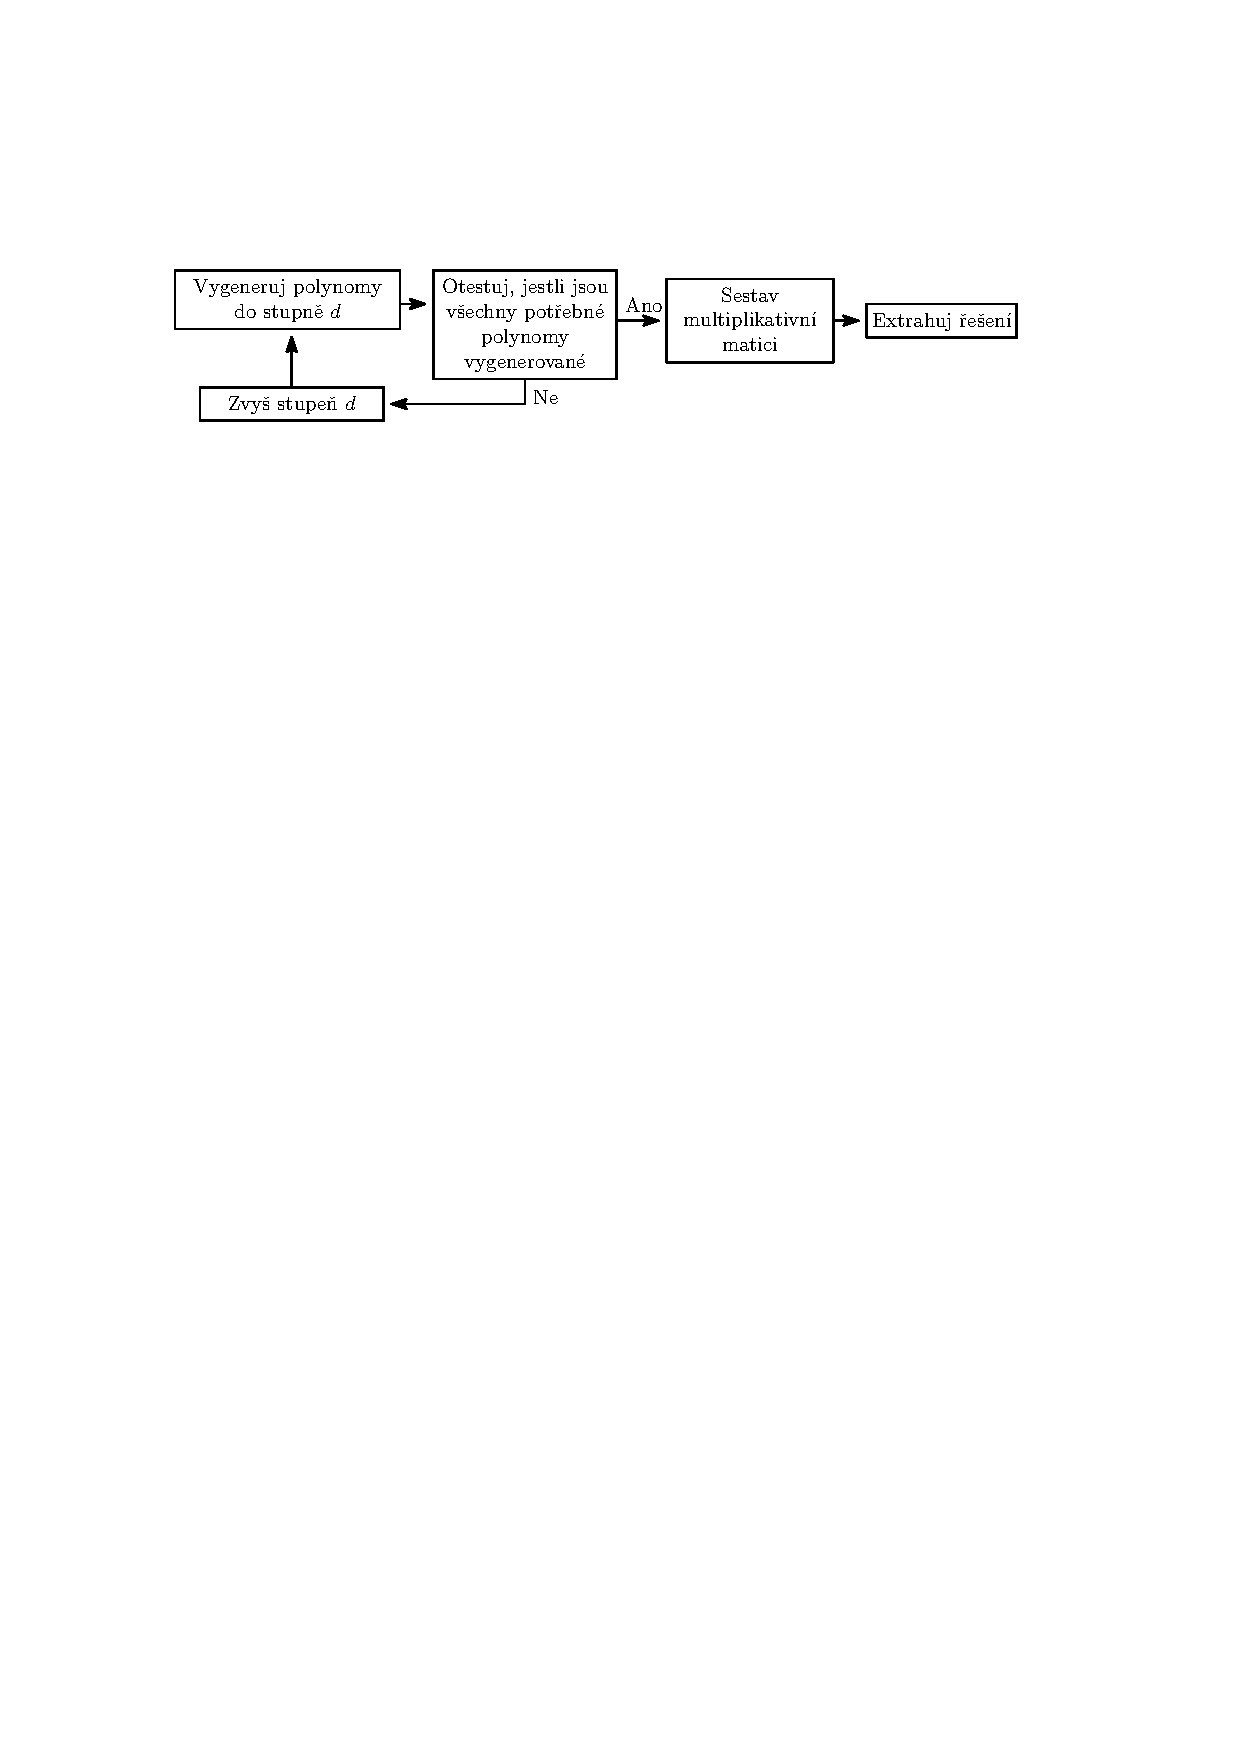
\includegraphics[width=25cm]{AutomaticGenerator-presentation.pdf}}
    \Put(0,0)[lb]{\footnotesize \cite{AutoGen} Z. Kukelova, M. Bujnak, T. Pajdla. Automatic generator of minimal problem solvers.}
  }

\end{cmptalkslide}

% --------------------------------------------------------------------------- 
\begin{cmptalkslide}[Víceeliminační postupy řešení]
  \begin{itemize}
    \item Polynomy generujeme systematicky, ale pravidelně je redukujeme pomocí Gauss-Jordanovy eliminace
    %\item Provedeme Gauss-Jordanovu eliminaci
    %\item Toto opakujeme dokud se generují nové polynomy
    %\item Zvýšíme stupeň generovaných polynomů o $d$
    \item Počet eliminací lze jednoduše řídit
    \item Efektivní zvláště pro soustavy s~velkým počtem neznámých
  \end{itemize}

  \placeat{
    \Put(.5,0.3){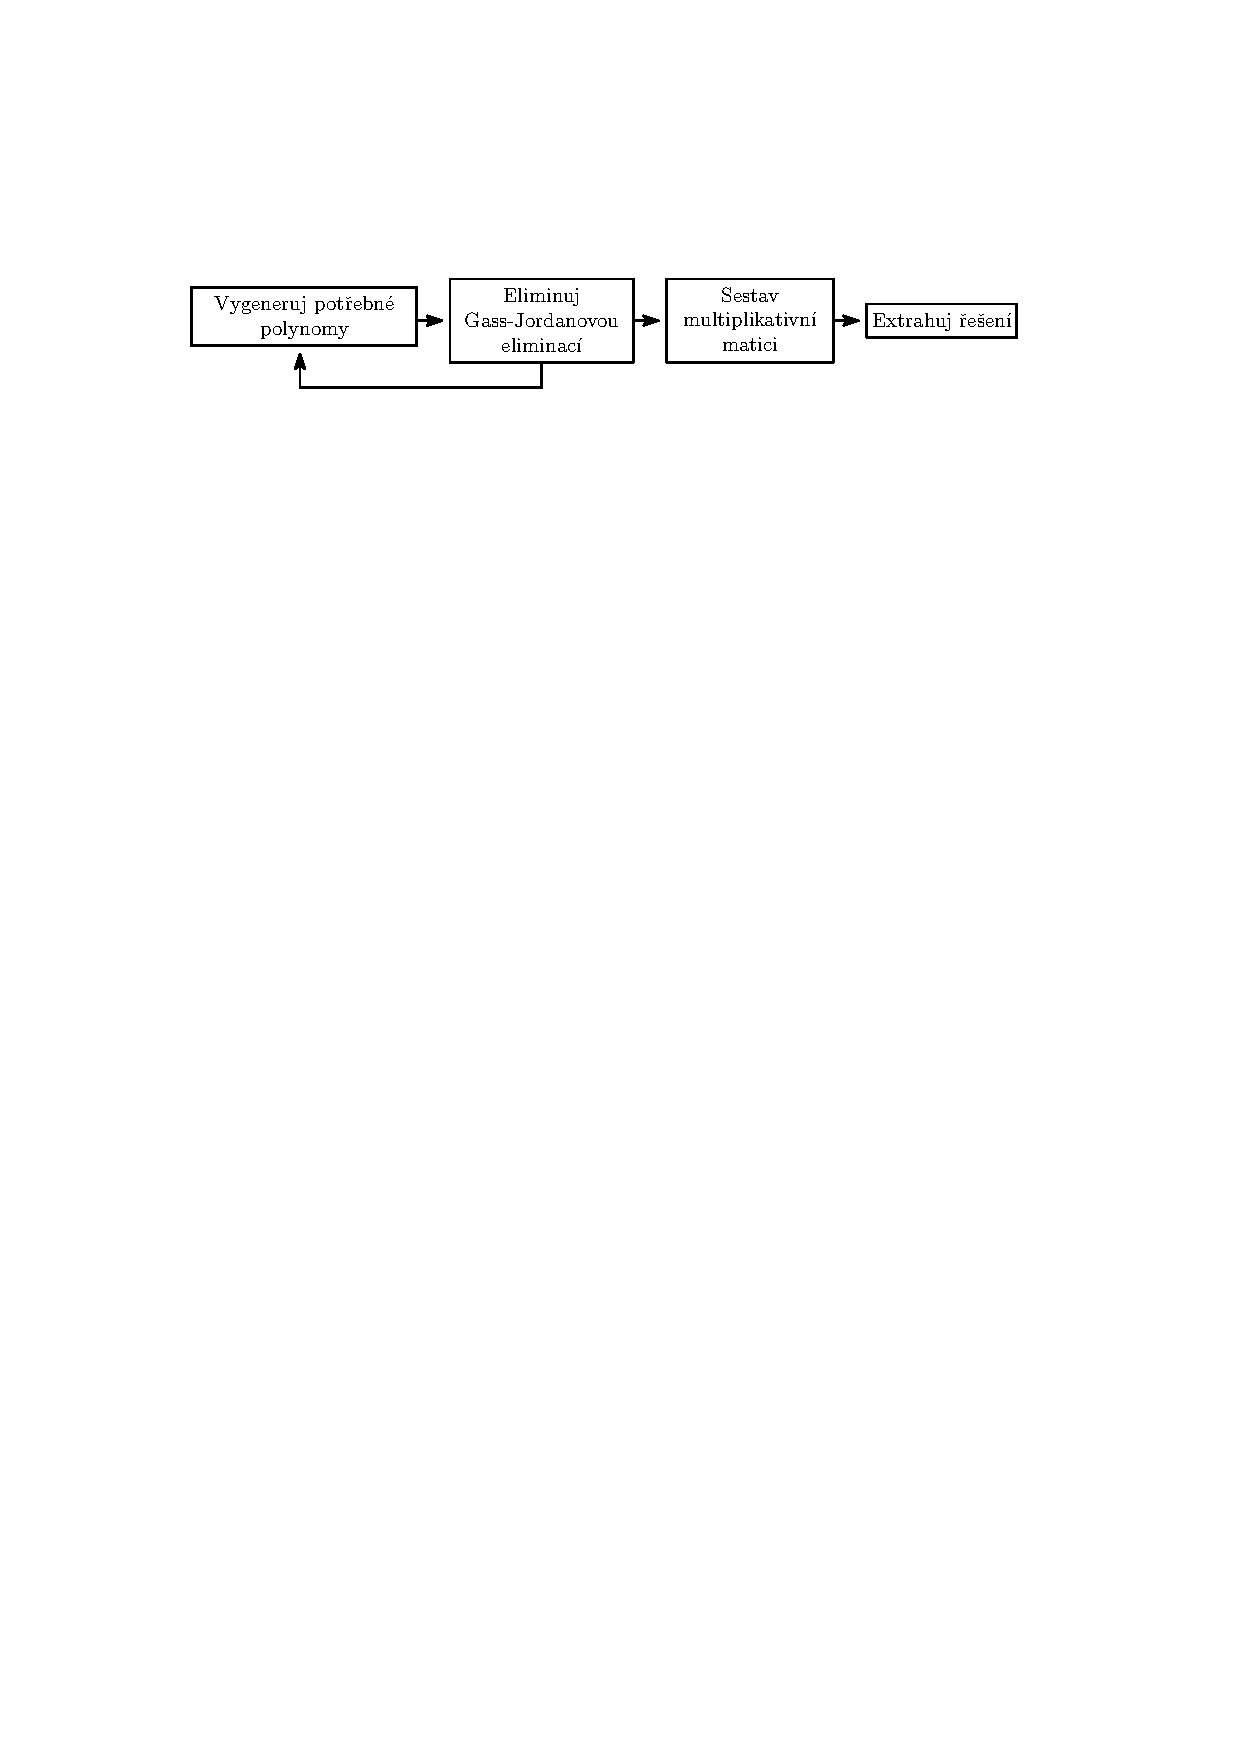
\includegraphics[width=25cm]{MultipleElimination-presentation.pdf}}
  }

\end{cmptalkslide}

% --------------------------------------------------------------------------- 
\begin{cmptalkslide}[Rozklad matic]
  \begin{itemize}
    \item Automatický generátor často pracuje s řídkými maticemi
    \item Snaha zrychlit Gauss-Jordanovu eliminaci řídkých matic
    \item Vycházeli jsme z poznatků \cite{SBBD}, že permutacemi sloupců a řádků lze matici převést do SBBD\footnote{Signly-bordered block-diagonal form} tvaru
    \item Poté lze provést dvě eliminace polovičních matic místo jedné eliminace celé matice
    \item Teoretické zrychlení je $n^3 \rightarrow 2\left(\frac{n}{2}\right)^3$
  \end{itemize}

  \placeat{
    \Put(.75,0.25){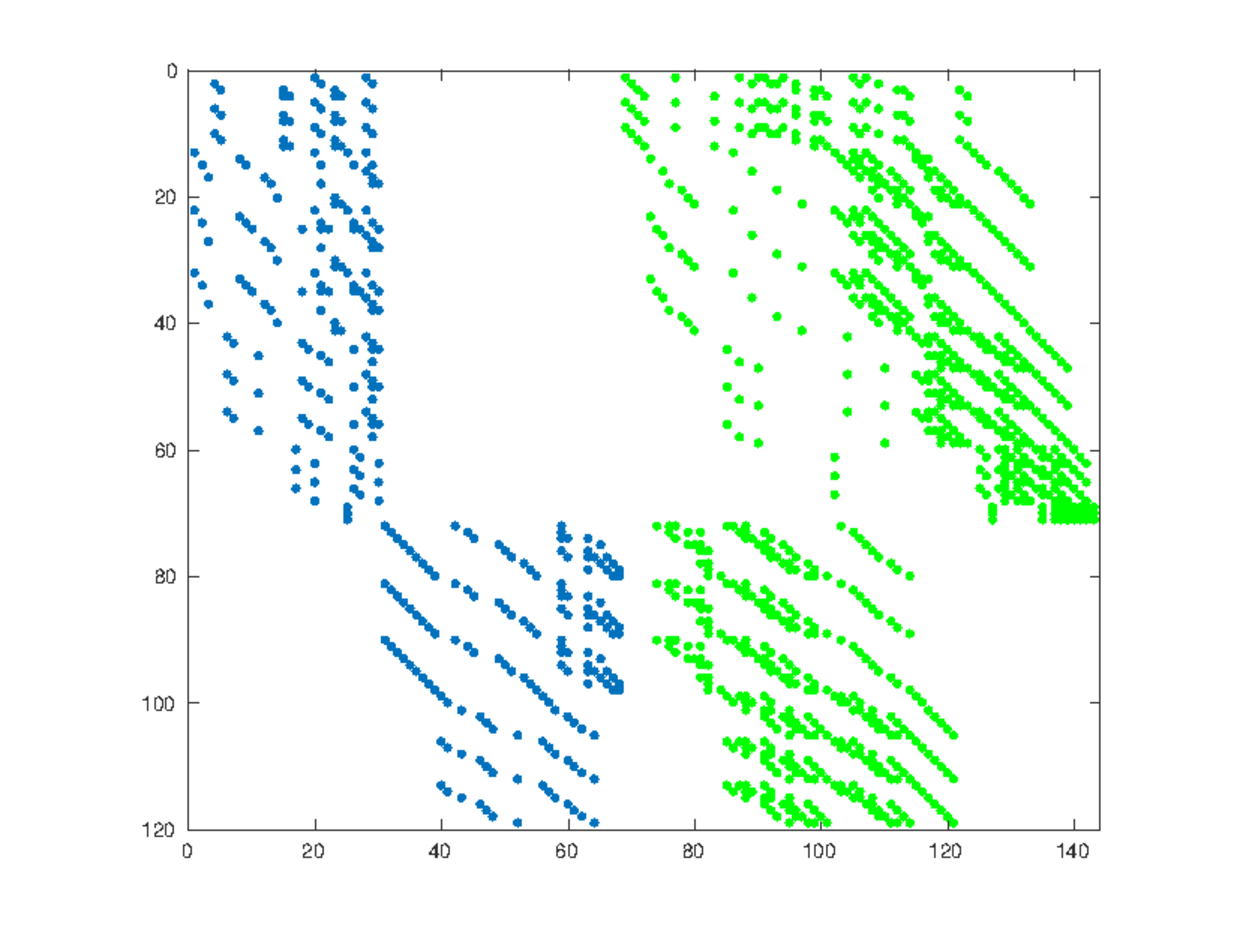
\includegraphics[width=14cm]{PaToH/permutation-presentation.pdf}}
    \Put(0.75, 0.49){\scriptsize{Nenulové prvky matice}}
    \Put(0.75, 0.01){\tiny{Sloupce}}
    \Put(0.54, 0.26){\rotatebox{90}{\tiny{Řádky}}}
    \Put(0,.15)[lb]{\footnotesize \cite{SBBD} Z. Kukelova, M. Bujnak, J. Heller, T. Pajdla.}
    \Put(0.03,.11)[lb]{\footnotesize Singly-bordered block-diagonal form for minimal}
    \Put(0.03,.07)[lb]{\footnotesize problem solvers.}
  }
\end{cmptalkslide}

% --------------------------------------------------------------------------- 
\begin{cmptalkslide}[Algoritmus $F_4$]
  \begin{itemize}
    \item Algoritmus $F_4$ \cite{F4} konstruuje Gr\"obnerovu bázi systému polynomů
    \item Nejprve jsme algoritmus implementovali v Maple, abychom jemu porozuměli a ověřili funkčnost implementace
    \item Algoritmus $F_4$ jsme implementovali do Automatického generátoru \cite{AutoGen}
    %\item Určuje, jak generovat nové polynomy
    \item Znalost Gr\"obnerovy báze umožňuje vygenerovat pouze potřebné polynomy
    \item Uživatel si může vybrat, zda se polynomy budou generovat systematicky nebo s využitím algoritmu $F_4$
  \end{itemize}

  \placeat{
    \Put(0,0.04)[lb]{\footnotesize \cite{F4} J.-C. Faugère. A new efficient algorithm for computing gröbner bases ($f_4$).}
    \Put(0,0)[lb]{\footnotesize \cite{AutoGen} Z. Kukelova, M. Bujnak, T. Pajdla. Automatic generator of minimal problem solvers.}
  }

\end{cmptalkslide}

% --------------------------------------------------------------------------- 
%\begin{cmptalkslide}[Benchmark Automatického generátoru]
%  \begin{itemize}
%    \item Z vygenerovaných potupů řešení různými metodami je třeba vybrat ten nejvhodnější pro danou aplikaci
%    \item Uživatel si zvolí, které metody chce použít pro generování postupů
%    \item Zadá testovací data, případně jsou benchmarkem vygenerována náhodná data
%    \item Automatický generátor vygeneruje požadované postupy řešení
%    \item Benchmark je otestuje na zadaných datech a porovná jejich rychlosti a stabilitu
%    \item Uživatel si vybere postup řešení, který je nejvhodnější pro danou aplikaci
% \end{itemize}
%\end{cmptalkslide}

% --------------------------------------------------------------------------- 
\begin{cmptalkslide}[Experimenty]
  \begin{itemize}
    %\item Postupy řešení vygenerované původní a novou implementací Automatického generátoru jsme srovnávali pro minimální problém "9-point relative pose different radial distortion problem" \cite{9pt}
    \item Testovali jsme na minimálním problému "9-point relative pose different radial distortion problem" \cite{9pt}
    \item Postupy řešení vygenerované novou implementací jsme srovnali s~původní verzí Automatického generátoru
    \item Víceeliminační postupy řešení: zrychlení 1,5$\times$, mírně zhoršená stabilita
    \item Posupy řešení s $F_4$ strategií: zrychlení 2$\times$, stejná stabilita
    \item Rozklad matic: další zrychlení o~20~\% v obou případech, numerická stabilita zachována
  \end{itemize}

  \placeat{
    \Put(0,0.04)[lb]{\footnotesize \cite{9pt} Z. Kukelova, M. Byröd, K. Josephson, T. Pajdla, K. Åström. Fast and robust numerical solutions}
    \Put(0.03,0)[lb]{\footnotesize minimal problems for cameras with radial distortion.}
  }

\end{cmptalkslide}

% --------------------------------------------------------------------------- 
\begin{cmptalkslide}[Shrnutí]
  \begin{itemize}
    \item Rozšířili jsme Automatický generátor \cite{AutoGen}
    \item Generuje postupy řešení s více eliminacemi
    %\item Umožňuje užít rozkladu řídkých matic a tím zrychlit Gauss-Jordanovu eliminaci
    \item Zrychlení Gauss-Jordanových eliminací pomocí rozkladu matic
    \item Implementace algoritmu $F_4$ \cite{F4} v Maple
    \item Možnost volby, zda se budou polynomy generovat systematicky nebo algoritmem $F_4$ \cite{F4}
    %\item Implementovali jsme benchmark Automatického generátoru
    \item Dosaženo dvojnásobného zrychlení generovaných postupů řešení pro vybraný problém \cite{9pt}
  \end{itemize}

  \placeat{
    \Put(0,0.12)[lb]{\footnotesize \cite{F4} J.-C. Faugère. A new efficient algorithm for computing gröbner bases ($f_4$).}
    \Put(0,0.08)[lb]{\footnotesize \cite{AutoGen} Z. Kukelova, M. Bujnak, T. Pajdla. Automatic generator of minimal problem solvers.}
    \Put(0,0.04)[lb]{\footnotesize \cite{9pt} Z. Kukelova, M. Byröd, K. Josephson, T. Pajdla, K. Åström. Fast and robust numerical solutions}
    \Put(0.03,0)[lb]{\footnotesize minimal problems for cameras with radial distortion.}
    \Put(.5,0.24){\large \textbf{Děkuji za pozornost}}
  }

\end{cmptalkslide}

% --------------------------------------------------------------------------- Bibliography
\begin{cmptalkslide}[Použitá literatura]
  \bibliographystyle{plain}
  {\small\bibliography{citations}{}}
\end{cmptalkslide}

% --------------------------------------------------------------------------- 
%\begin{cmptalkslide}[]
%  \begin{center}
%  \vfill
%  {\Large \textbf{Děkuji za pozornost}}\\[5cm]
%  {\large \textbf{Prostor pro vaše otázky}}
%  \vfill
%  \end{center}
%\end{cmptalkslide}


\end{document}
